\chapter{Projectgrenzen}
In dit hoofdstuk worden de projectgrenzen toegelicht.
De afbakening van het project licht toe wat er wel en niet gemaakt binnen de context van de afstudeeropdracht.
Vervolgens wordt de definition of done beschreven om aan te tonen wanneer de opdracht voldaan is.
Daarna worden de randvoorwaarden van de afstudeeropdracht besproken.
\section{Afbakening}
%
% wat wil ik zeggen 
% - Het huidige Snakware cloud platform is erg groot en kunnen nooit alles maken dat het platform klan
% - Het huidige platform bestaat uit 3 verschillende applicaties: CMS-API, de Snakeware cloud frontend , de klant zijn web applicatie.
% - wat er wordt gemaakt is de de CMS-API en de klant zijn webapplicatie te de content tonen
%
Het huidige Snakware cloud plaform heeft in de loop der jaren veel functionaliteiten gekregen.
Hierom is het van belang dat tijdens de afstudeerperiode de opdracht niet te groot wordt gemaakt om het succesvol te kunnen afronden.
Daarom wordt er primair gefocust op het realiseren en ontwerpen van de CMS-API.

\whitespace[2]
Snakeware cloud bestaat momenteel uit 3 verschillende applicaties, deze applicaties zijn:
\begin{itemize}
    \item[-] Snakeware cloud \gls{GUI}  
    \item[-] CMS-API
    \item[-] klant webapplicatie
\end{itemize}

\whitespace[2]
Er is besloten om niet de Snakeware cloud \gls{GUI} te maken om de scope van de afstudeeropdracht haalbaar te maken.
Daarnaast wordt de klant webapplicatie minimaal uitgewerkt om de data van de CMS-API te kunnen tonen.
Om de \gls{UserJourneys} te kunnen valideren worden ze getest door middel van postman workflows.
Voor verheldering is in figuur \ref{fig:ProductOverview} een versimpelde communicate diagram van de producten die gemaakt en niet gemaakt worden tijdens de afstudeer opdracht.\\
\begin{graphic}
    \vspace{0.2cm}
    \captionsetup{type=figure}
    \caption{Gesimplificeerde communicatie diagram van  systemen}
    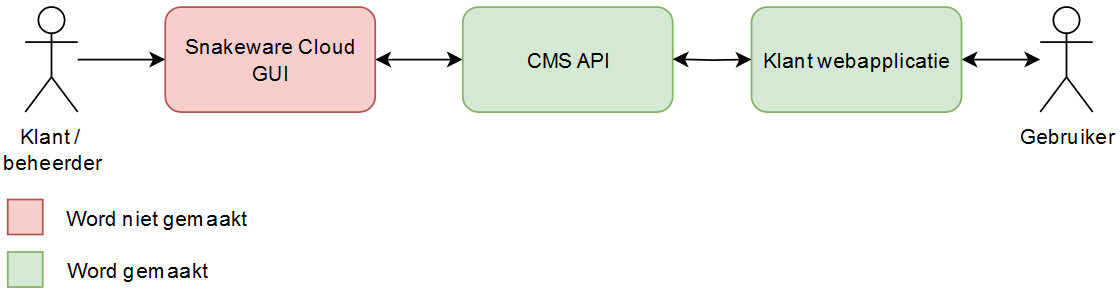
\includegraphics[scale=0.4]{ProductCommunicate}
    \label{fig:ProductOverview}
    \vspace{0.2cm}
\end{graphic}

\section{Definition of done}
De definition of done is wanneer er een proof of concept \gls{CMS}-API en de daarbij behorende klant webapplicatie is opgeleverd. 
Die voldoen aan de belangrijkste (de must have’s van de MoSCoW analyse) eisen en wensen die uit het onderzoek zijn gekomen van de stakeholders.
Het systeem moet flexibel opgesteld worden, zodat in de toekomst extra functionaliteiten toegevoegd kunnen worden.
Daarnaast is het van belang dat de school documentatie met een voldoende wordt afgerond.
De verschillende documenten zijn: plan van aanpak, onderzoeksverslag en het technisch verslag.
Daarnaast moet het product en de presentatie met een voldoende afgerond worden.

\section{Randvoorwaarden}
Om het project goed af te kunnen ronden zijn er randvoorwaarden aan het project verbonden:
\begin{itemize}
	\item[-] Er is een werkplek nodig om alle werkzaamheden tijdens de afstudeerperiode te kunnen afronden.
	\item[-] Er wordt een keer per week een afspraak gemaakt met de bedrijfsbegeleider en de docentbegeleider om de progressie te bespreken.
	\item[-] De afstudeeropdracht moet afgerond worden binnen de duur van de afstudeerperiode.
	      Dit is ongeveer 125 werkdagen en loopt van 18 november 2023 tot 5 april 2024.
\end{itemize}



